\documentclass[./../../paper.tex]{subfiles}
\graphicspath{{\subfix{./../../figures/}}}

\begin{document}
As explained earlier, we run the same configuration as previously established for this simulation. However, we vary the rate with which we apply a mutation type this time. 

\begin{figure}[htbp]
    \centering
    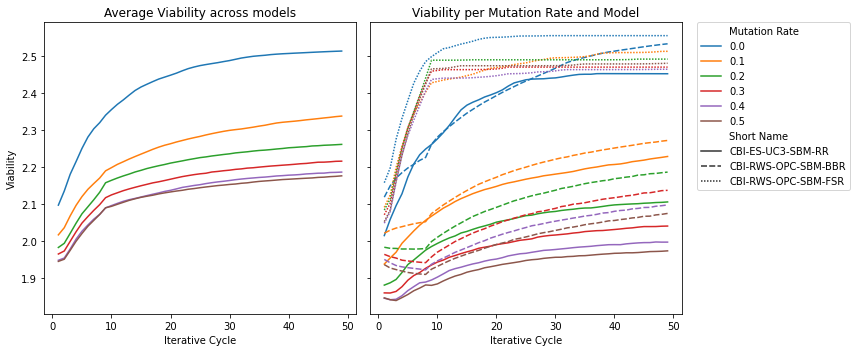
\includegraphics[width=\textwidth]{figures/generated/exp2_viability_by_mrate_model.png}
    \caption{This figure shows the viability for each model and mutation rate per iterative cycle. The first plot shows the average across models. The second figure shows the same information per model. The x-axis shows how the viability evolves for each evolutionary cycle. The colour indicates the mutation rate. The line-type marks each model tested.}
    \label{fig:average-mutation-rates}
\end{figure}


\noindent As we can see in \autoref{fig:average-mutation-rates}, a mutation rate of 0 yields better results on average. We are suggesting that mutating the children might impede the model. 
For model configurations that use the Fittest-Survivor-Recombination, we observe a sharp pattern of convergence before the 10th iterative cycle.  

% \graphicspath{{\subfix{./../../figures/}}}

\begin{figure}[htbp]
    \centering
    \begin{subfigure}[c]{0.49\textwidth}
        \centering
        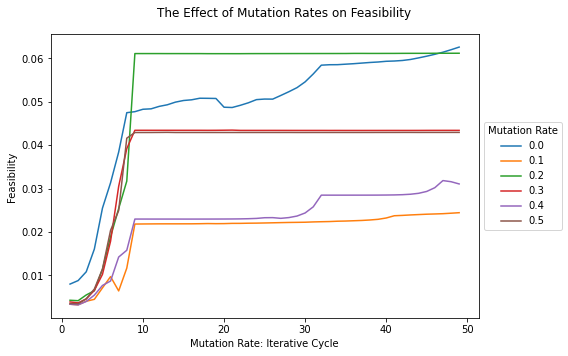
\includegraphics[width=\textwidth]{figures/generated/exp2_feasibility.png}
        \label{fig:exp2-feasibility}    
    \end{subfigure}
    \hfill
    \begin{subfigure}[c]{0.49\textwidth}
        \centering
        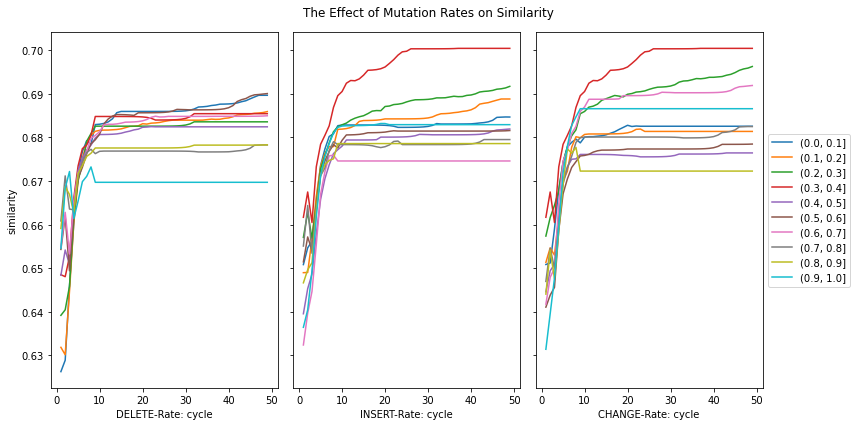
\includegraphics[width=\textwidth]{figures/generated/exp2_similarity.png}
        \label{fig:exp2-similarity}
    \end{subfigure}
    \hfill
    \begin{subfigure}[c]{0.49\textwidth}
        \centering
        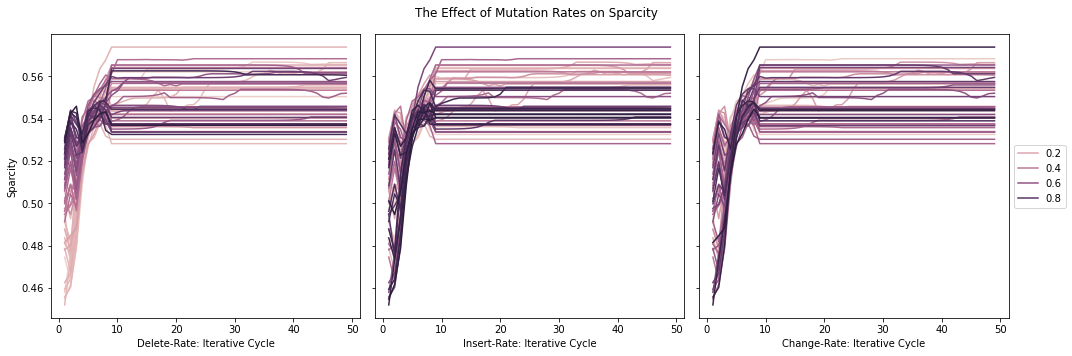
\includegraphics[width=\textwidth]{figures/generated/exp2_sparcity.png}
        \label{fig:exp2-sparcity}
    \end{subfigure}
    \hfill
    \begin{subfigure}[c]{0.49\textwidth}
        \centering
        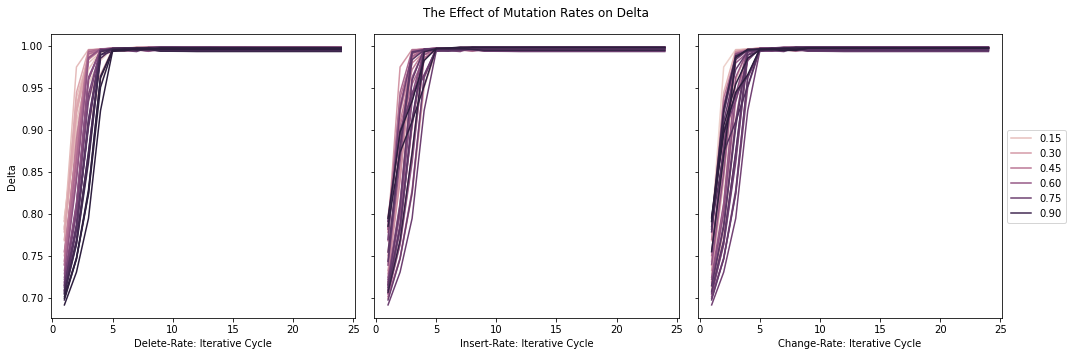
\includegraphics[width=\textwidth]{figures/generated/exp2_delta.png}
        \label{fig:exp2-delta}
    \end{subfigure}
    \caption{Shows all components of the viability measure.}
    \label{fig:exp2-measure}
\end{figure}

\autoref{fig:exp2-measure} reveals the reason for this behaviour.
In all plots of a sharp change right before the 10th iterative cycle. However, the feasibility measure also displays a sudden stop of improvement for all mutation rates except 0.0 and 0.4. These exceptions also change their growth rate but improve shortly after the 30th iterative cycle. The figure also shows that a mutation rate of 0.2 reaches the highest feasibility among the other edit rates. However, after 48 cycles, the mutation rate of 0.0 overtakes 0.2.     

\end{document}